\section{Introduction}
% Main Ideas:

% IEAs
% Human Based Computation
% C-IEAs
% Problems
% Volunteers 
% Human Centered
% C-IEA Complex Interactions
  % User -> Human
  % Social Network
  % Devices IoT
  % Activities
  % Engagement

% Why an HC Framework (Objectives)  
% Presentation 


% IEAs
Interactive evolutionary computation (IEC) systems are, in general, evolutionary methods
whose fitness evaluations are performed by humans through an
interactive system \cite{eiben2015interactive}. They are usually
applied in problems where the fitness function is not known  or simply
does not exist, and the result
of optimization should fit certain human and possibly aesthetic
need. That is why their use case includes the evolution of objects
with subjective characteristics such visual appeal or 
attractiveness \cite{biomorphs} as well as others where human behavior is 
considered, for instance to optimize teamwork \cite{kosorukoff2002evolutionary}
or creativity cite[cook].
% Human Based Computation
These IEC systems are an interesting venue of research, since they have demonstrated their ability for effectively 
producing art and design \cite{Bentley:1999:intro,Sims:1991,todd:1992,evoeco},
as well as other artifacts in many other domains \cite{ie1}. In these cases when human interaction is responsible of other 
operations of the evolutionary process some authors classify these IEC methods 
as human-based evolutionary computation cite[kosorukoff] or as human-based computation cite[].

% C-IEAs
One of the issues with these systems is that their performance effectively depends on the number of users
they are able to include; and in order to reach more human users,
Interactive Evolutionary Algorithms (IEAs) are 
some times developed as web applications depending on visitors to the web to interactively help
with the search, using both anonymous and registered users. Some systems 
employ a collaborative technique, where several users assign a quality assessment 
to a single solution and then an aggregated fitness value is calculated 
\cite{picbreeder,seyama2016development,wagy2014collective}.
% Problems
However, the necessary intervention of humans in these systems leads
to them having several inherent problems arising from the very nature of 
the algorithms, namely, human evaluations are slow and expensive, there is a
human fatigue caused by the interaction \cite{ie1}, and
the boredom arising when users evaluate a large number of phenotypes 
many of which are not interesting or are very similar to each other. 
The number of evaluations that IEC can receive is limited by the number of users
collaborating and the amount of interaction of each. Having a volunteer system 
can lower the requirements of anyone participating in
the experiment thus increasing the {\em performance}, in terms of {\em
human brain cycles}, of the whole system.
% Volunteers 

Using a volunteer based system raises other issues \cite{sarmenta2001volunteer,web:BOINC}, 
such as the volunteer\'s lack of accountability,
and the need to build trust between participants and application
providers. Issues for the provider of the system or organizer  are also the difficulty of establishing 
the amount of time and resources
a volunteer is willing to spend on the system, and how they decide if they
participate or not \cite{JJ:2016}. 

% Human Centered
In order to increase volunteer participation and to tackle some of the issues mentioned above,  
we proposed a framework following a human centered design \cite{greenhouse2012human},
giving extensive attention to volunteers, not only because their
explicit evaluation is essential, but also because the context of the 
interaction affects the system as a whole. In collaborative systems, users interact 
with each other, and are aware of the actions ref[]. Users also consider their previous evaluations
and past experiences ref[].

%Please help with this paragraph, is evidence needed?
% It's the tuning of the algorithm which is data driven, not the
% algorithm itself, right? - JJ
%  Tuning yes - Mario
% And evidence for what? - jj
%  That most EAs use only population data - Mario
In evolutionary computation algorithms are data driven since it is important to keep data about the 
population of each generation, in order to generate the next or even change certain parameters
or analyze the evolutionary process. 
% Human Centered Importance
The framework models the context of interaction along with the population and
this knowledge is available to be an integral part of the evolutionary computation.
%This could be generalized?
For example, in a C-IEC application, fitness assignment depend on the
actions of a social network of users. 
A stream of actions is triggered when they tag, share, rate, store or even delete a phenotype. 
The selection of parents could also depend also on the previous actions, leveraging information 
such as the fact that they have the same tag, or are shared by
similar users. That knowledge could also be applied in choosing which phenotypes present to a certain
users, in order to give them those they will find more interesting or useful. 
% IoT
The context of interaction, can also include data retrieved from sensors and other IoT devices.
% Engagement
Data available from the interaction is also used to increase the performance of the system by applying 
gamification techniques. Gamification is defined by Deterding et al. as
``the use of game design elements in non-game contexts'' \cite{deterding2011game}.
The gamification element employed in a case study is a rewarding mechanism  
\cite{dubois2013understanding}, in general they consist of a reputation system with score points, 
levels and leader boards. Points are awarded to users in response of 
the accomplishment of certain activities that need to be encouraged. Levels depend
on the score and certain features of the game are only available to gamers when 
they reach a giving level.

Three case studies are presented as a proof of concept, providing both
conceptual and implementation details of the framework. 
The experiments were implemented using the EvoSpace-Interactive framework \cite{garcia2013evospace}, 
and where employed in different contexts of interaction. 
Additional details of each case study application is presented elsewhere refs[][][]. 
Giving this paper the objective of presenting the underlying conceptual framework.     

The rest of this paper is organized as follows.
Section \ref{sec:interactive} presents related work on the topic 
of Interactive Evolution.
Then, Section \ref{sec:e} presents the Model of Human Interactions in Collaborative Interactive 
 Evolutionary Computation which 
the main proposal of this work. An implementation using the EvoSpace-Interactive  framework is detailed in Section \ref{sec:HCF}.
The case studies  and results are presented in Section \ref{sec:experiments}.
Finally, a concluding remarks are provided in Section \ref{sec:conclusions}.

\section{Related Work}
% C-IEAS
% Volunteer Based
% HBC
% Engagement Techniques
% Models

\begin{figure*}[!t]
    \centering
        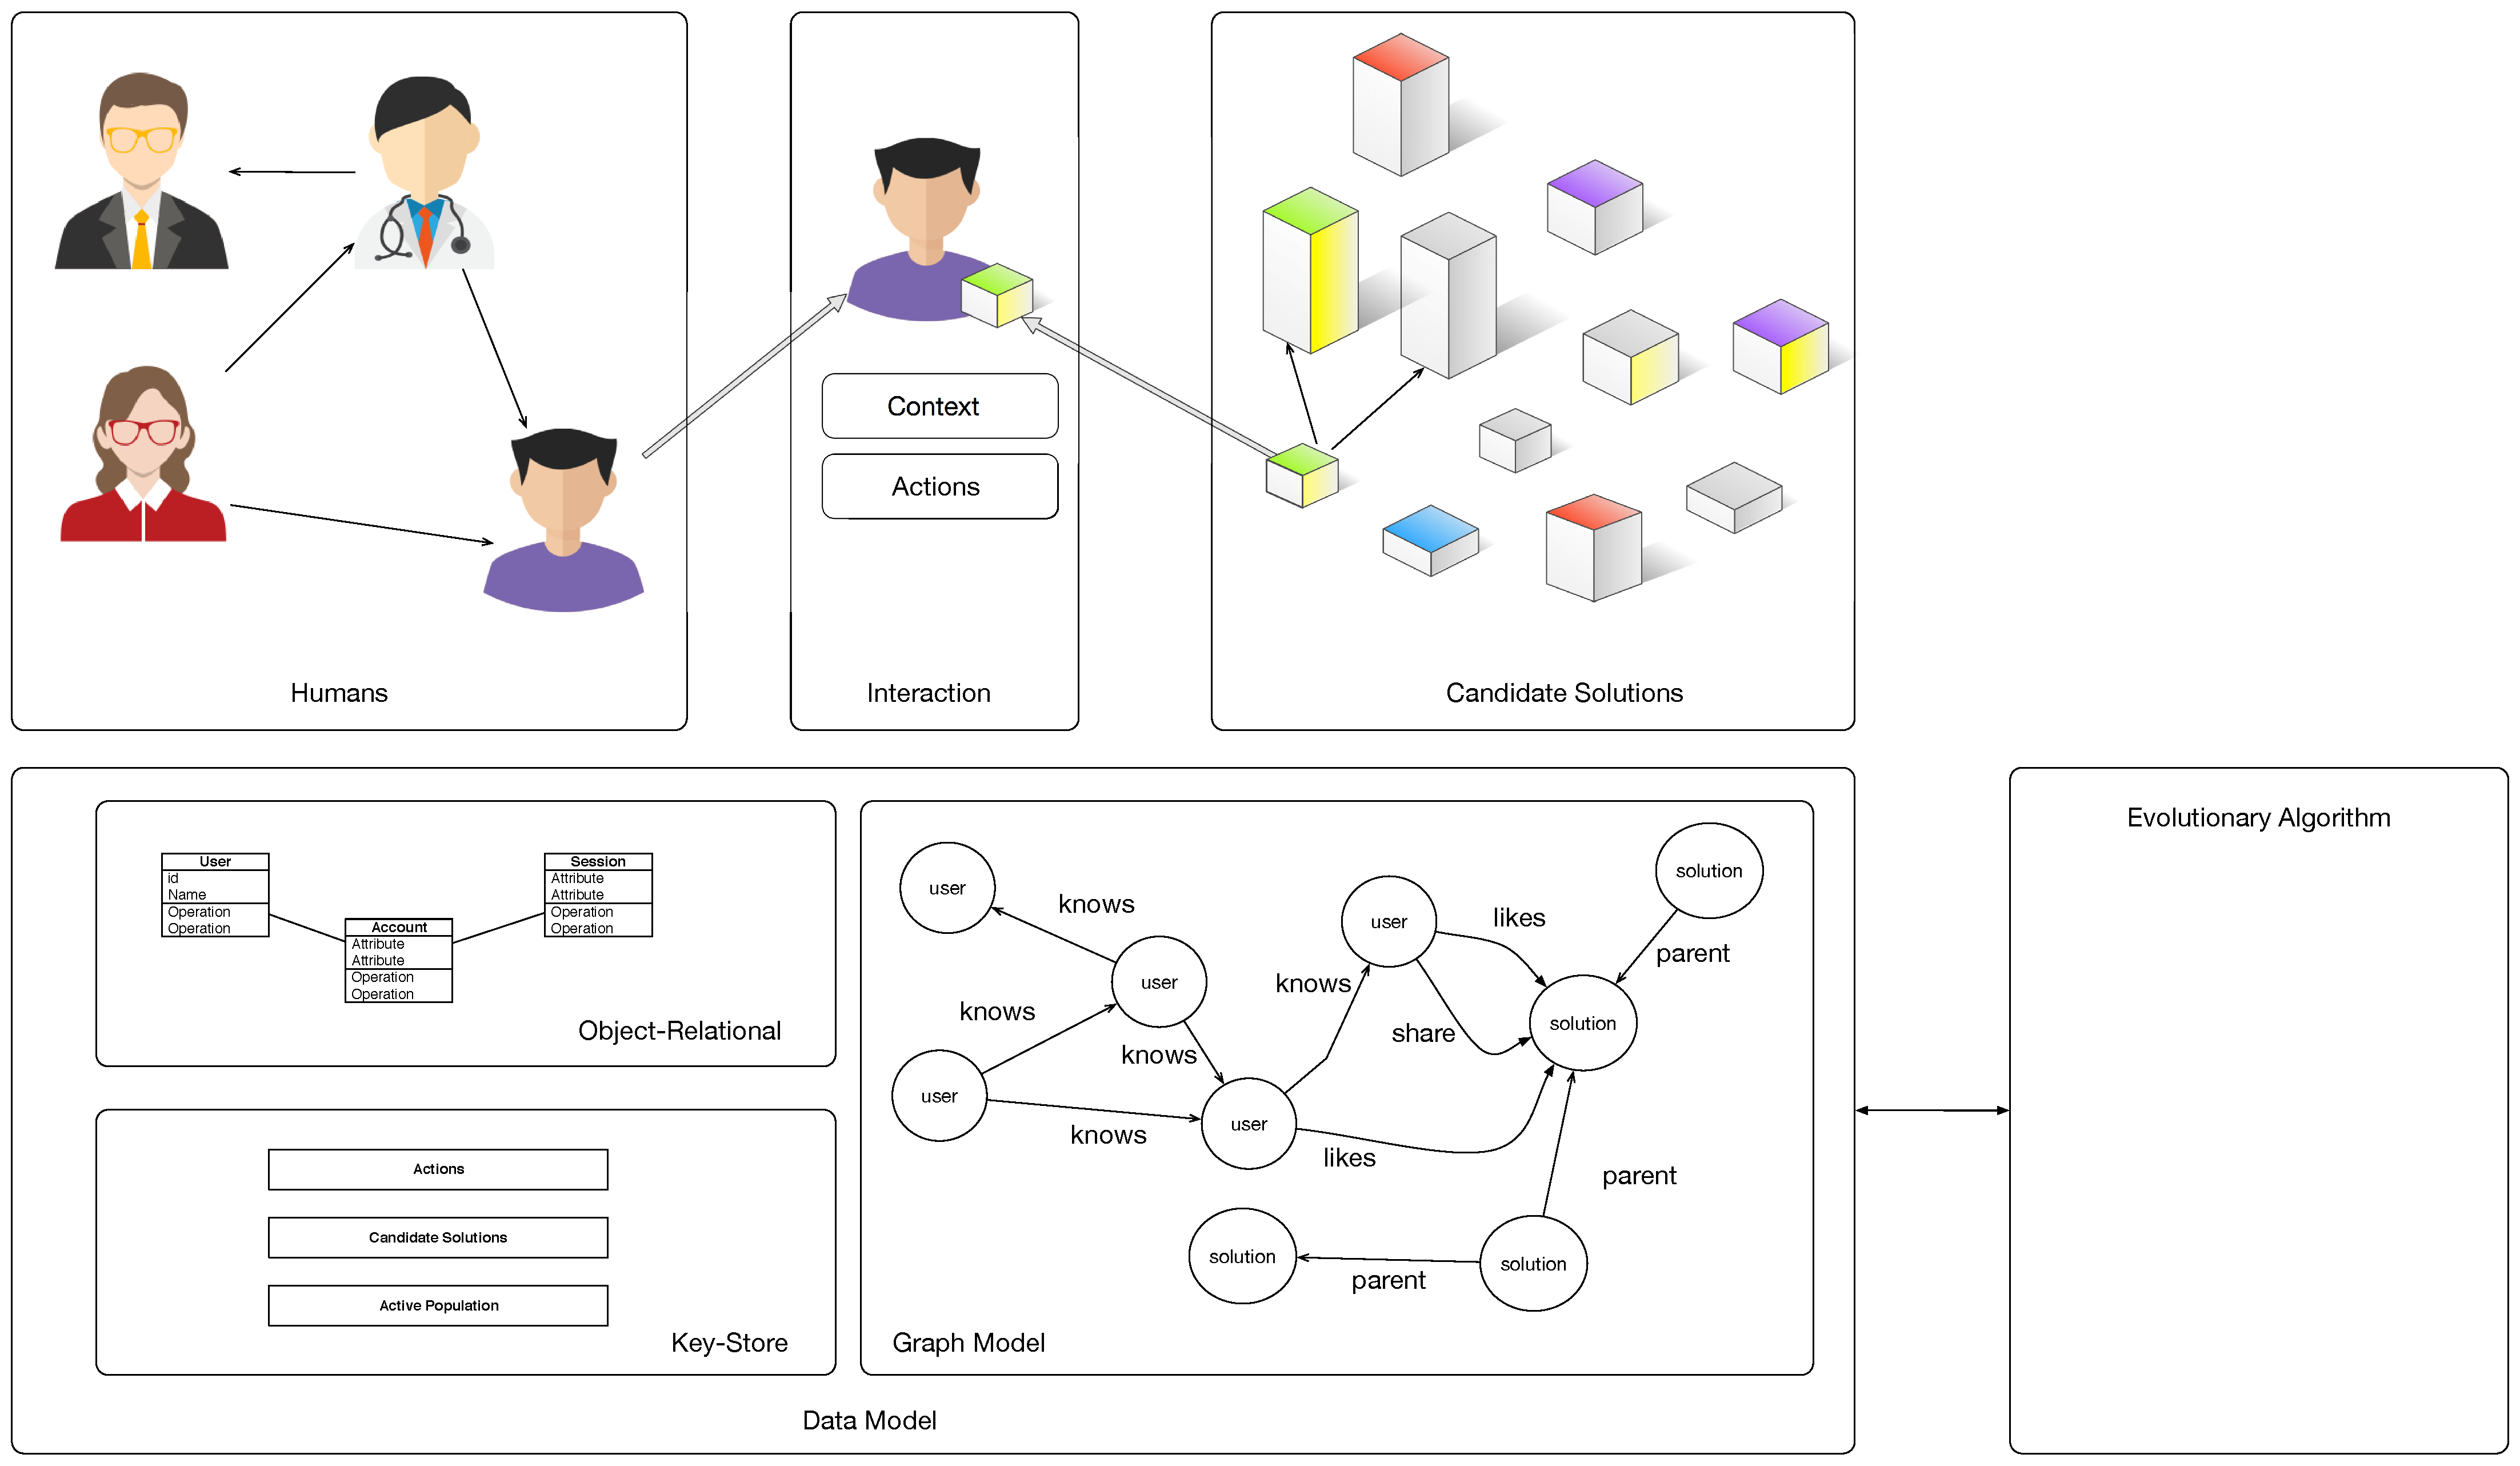
\includegraphics[width=4.5in]{img/framework.eps}
    \caption{IEC Human-centered framework.}
    \label{fig:uc_framework}
\end{figure*}

\section{Human-Centered IEC Framework}
% Comment: 
% Maybe in this case we should use the term software framework or architecture. 
The general goal of this research is to develop a human-centered \cite{gasson2003human} 
software framework for interactive evolutionary computation (IEC). 
The framework is a reusable architectural design together with an implementation \cite{campbell1991choices}, 
providing generalized components to developers of IEC systems. In the description we deliberately use the more general 
term Human instead of User, because humans are not always playing the role of users in software engineering sense, they
could just be interacting naturally with their environment and with out knowing they are implicitly
evaluating a possible solution. The framework includes components that can be refined to increase
participation and also to minimize the amount of evaluations needed for the evolutionary process in a given IEC application. Software frameworks often have a vison or a way of thinking \cite{carneiro2010introducing} guiding their
design. Before entering to details the main design decisions of the framework are explained next:  

\begin{itemize}
\item {\bf Users are human} 
  The framework follows the approach of human centered computing \cite{sebe2010human},
  in which the context, environment, interfaces, preferences, accessibility, human relations, cognitive
  limitations, culture, creativity and other human aspects are an integral part of the system.
  Humans are the computing resorces of the system, having unique characteristics as those identified by 
  Sun \& Dance \cite{Sun2013}  ``(1) humans can solve computer hard problems; (2) humans are very good at exception handling, (3) humans have creativity, (4) humans have cognitive load limitation, (5) humans are vulnerable to 
  psychological manipulation, (6) humans are prone to errors, especially for reflective tasks.''


\item {\bf Users are volunteers} Users donate their computing resources, so they are unaccountable, 
  some times they try to game the system. Providers must actively promote and design the interactive
  system to engage volunteers \cite{oh2015clicking}. 

\item {\bf Users are not alone}
  Relationship between users in an interactive evolutionary algorithm can be modeled
  as a social network, with well established semantics, algorithms and metrics \cite{ahuja1993network}.
  A graph model could enable researchers to find other ways of identifying leaders of 
  opinion or measuring the similarity between user's preferences. 
  These measures can then be used by recommender algorithms selecting 
  phenotypes according users' preferences. 

\item {\bf Context of use matters}
  \textit{Context} In computer science Fischer \cite{fischer2012context}
  defines context as \textit{``the interaction between humans and
  computers in socio-technical systems that takes place in a certain
  context referring to the physical and social situation in which
  computational devices and environments are embedded"}. 
  Fischer also identifies the important aspects to consider when the context is used: how it is
  the contextual data obtained, how the context is represented and what
  goals and purposes the context has when is used in a particular
  application.   An IEC system will  be used within a certain range of technical, physical and social or
  organizational environments \cite{maguire2001context} that may affect its use.
  The concept has been formally defined
  by ISO standard 9241-11 \cite{international1998iso} as \textit{``users,
  tasks and equipment (hardware, software and materials), and the
  physical and social environments in which a product is used"}.  

\item {\bf Interaction is a stream of actions}
  Real time processing of users' actions could be needed for certain applications when data is 
  captured by sensors, or directly captured as user input. For example, social networks keep track of 
  users' interactions with other users, media objects and places. Users of 
  social networks (for instance the Facebook Graph) are accustomed to express these 
  complex relationships in sentences such as: ``John and Ann eating breakfast at Tony's''. 
  Other example is the W3C Activity Streams 2.0 specification used for representing activities 
  common in social web applications \cite{json:streams}. 
\end{itemize}

The human centered IEC architecture consists of three high level components depicted
in figure \ref{fig:uc_framework}:

\begin{itemize}
  \item {\bf Interactive Evolutionary Computational system} 
  This is the real world system that we are going to represent in the data model, 
  it consist of human users and their interactions with one or more phenotypes
  from the population. There are many ways in which humans could interact 
  with phenotypes. The interaction consists of a set of actions and 
  takes place in a certain context. For example, through a mobile device  
  or by interacting with real world objects 
  \cite{de2014artists,de2013unplugging}. 
  There is also the possibility that fitness or even part of the search 
  is done by devices lent by humans \cite{DBLP:conf/gecco/MereloCGCRV16}.
  The information gathered through the interaction is the primary concern
  as it will guide the search. 

  \item {\bf IEC Data Model}
  A data model is used to describe the IEC system prior to a physical 
  implementation.  Depending on the domain several techniques can be used.
  Parts of the system could be better described by an Entity relationship 
  modeling to be used in a relational database or a class digram for a 
  key-value store. A graph is proposed for modeling the social network of users 
  and their interaction with the population. When implemented a graph database 
  will be the back-end of the system. 

  \item {\bf Evolutionary Algorithm} 
  The EA algorithm interacts with the data model. The EA could also be done with the help of
  humans, for instance in the XY project \cite{de2013unplugging} artists actually painted
  the solutions of the new population.  
\end{itemize}

\section{Data Model Implementation}
The core of the framework is the data model because both the IEC system and the EA will 
depend on the application. In this section implementation details of the Data Model are presented. 
  \subsection{EvoSpace}
  \subsection{Graph}
  \subsection{PostgreSQL}

  \subsection{Interfaces}
    
  \subsection{Evolution}



\section{Data Model Implementation}





\section{Case Studies}
\label{sec:evospace-i}
\begin{figure}[!t]
    \centering
        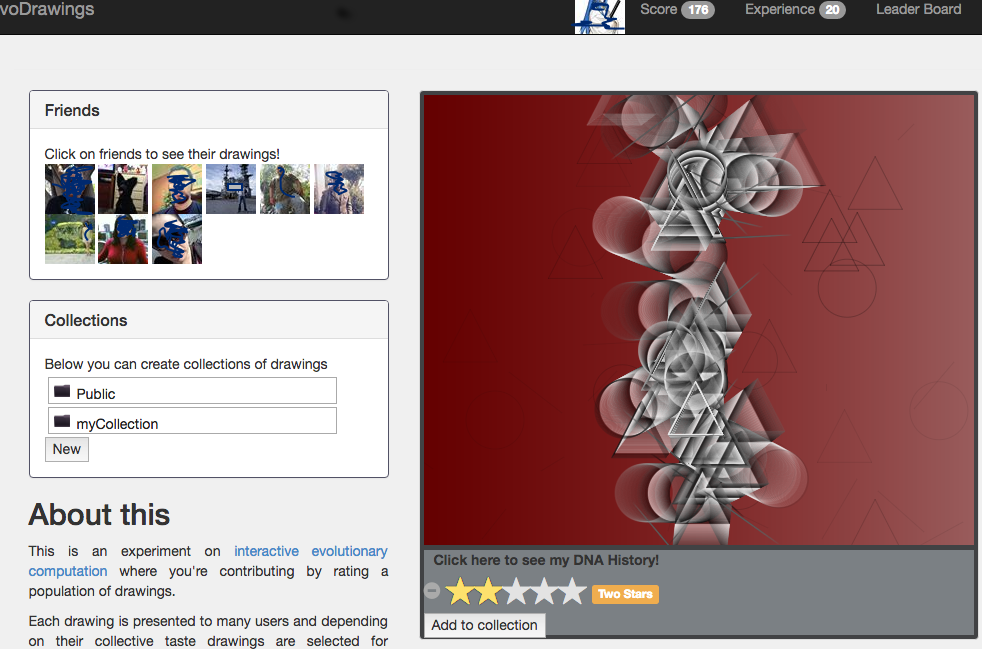
\includegraphics[width=3.5in]{img/interface.png}
    \caption{User interface of the EvoDrawings application.}
    \label{fig:web}
\end{figure}

\subsection{EvoDraw}
As a case study, a IEA was developed using the 
EvoSpace-Interactive (ES-I) platform \cite{garcia2013evospace}
A brief description of the application is presented next, focusing
on the data elements that where ported to the graph model.

\subsection{Fitness Assignment}
\label{sec:assignment}
The ES-I platform employs a collaborative technique,
where several registered users assign a quality assessment to a single
phenotypes and then an aggregated fitness value is calculated. The fitness
assigned to each phenotypes depends on the taste of each particular user, 
resulting in a many-to-many relationship between users and phenotypes. 
Many systems query this user-phenotype relation to extract relevant
knowledge about the process and the population, for instance showing the
most popular phenotype, or the the user with more participation 
\cite{picbreeder}.
In order to do this, data about phenotypes 
must be permanently stored, even
if they are no longer in the active population. 

\subsection{Collaboration}
\label{sec:col}
After entering the web application by using their Facebook account,
users can collaborate with their Facebook friends, 
sharing those phenotypes they like, or by taking phenotypes
from their friend's collections by using the web interface depicted 
in Figure \ref{fig:web}.
At the top left corner a list of Facebook friends is presented
to encourage users to interact with the system. In the central 
\emph{ Wall } area, a phenotype sampled from the population that is
being evolved via the evolutionary algorithm 
is shown to the user.
Here, the user can interact with the system in two ways.
First, he can assign a quality assessment to the phenotype using
a five star rating system or,
additionally, a user can choose to add an image to one of their \emph{Collections}.
A collection is a special folder that stores those phenotypes a user likes and wishes
to save. After the user finishes interacting with the phenotype
on the Wall, he can choose to retrieve a new one from the population.
At the left hand side, the web page shows the \emph{Collections} section.
The user can create several collections, to group and organize his favorite 
artifacts. Moreover, users can browse the content of each collection and from
there share images through their social network.
When a user hovers the cursor over a phenotypes a pop-up pane shows how many users have
liked the phenotype. The pane also includes a link to the phenotype's 
details, the parents, genetic operators that created it, and genealogy
information. This makes the assignment of fitness through the rating
system a {\em social} activity, pursuing the objective of this work,
which is to increase engagement of the users.
\subsubsection{Graph Model} 
\subsubsection{Human Interaction Model}

\subsection{EvoDraw-Kinect}
\subsection{XYZ-Unplugged}


\section{Conclusions}

\begin{acks}
  % The authors would like to thank Dr. Yuhua Li for providing the
  % matlab code of  the \textit{BEPS} method. 

  % The authors would also like to thank the anonymous referees for
  % their valuable comments and helpful suggestions. The work is
  % supported by the \grantsponsor{GS501100001809}{National Natural
  %   Science Foundation of
  %   China}{http://dx.doi.org/10.13039/501100001809} under Grant
  % No.:~\grantnum{GS501100001809}{61273304}
  % and~\grantnum[http://www.nnsf.cn/youngscientsts]{GS501100001809}{Young
  %   Scientsts' Support Program}.

\end{acks}
